\section{Results}
\label{sec:results}

Unless stated otherwise, estimates are at the frozen 80\% cutoff with
impression-derived labels and $T=3$. Intervals are 95\% patient-clustered
percentile intervals. ``Original'' denotes the estimator used in the previous
draft and ``corrected'' the evaluable-study estimator (\cref{sec:endpoint}).

\subsection{Cohorts and what the labels cover}
\label{sec:res-labels}
The source evaluation cohort comprised 14,766 studies (16,456 images, 5,000
patients), all informative by construction. The external cohort comprised
\ExtStudies{} studies (\ExtImages{} images, \ExtPatients{} patients), of which
\ExtNOne{} were informative (N1), \ExtNTwo{} low-information (N2) and \ExtNThree{}
absent (N3). The N1 subset (\ExtNOneImages{} images, \ExtNOnePatients{}
patients) is the external intervention cohort.

Label coverage differed sharply between sites (\cref{tab:labels},
\cref{fig:labels}). Under impression-derived labels, \NoLabSrcImpression{}
(\NoLabNSrcImpression{}) of source studies and \NoLabExtImpression{}
(\NoLabNExtImpression{}) of external studies had no positive or negative label
for any of the five targets. Labelled-cell density was \DensSrcImpression{}
versus \DensExtImpression{}, and the positive rate among labelled cells
\PosSrcImpression{} versus \PosExtImpression{}. Similar aggregate positive rates
concealed different compositions. The external site carried far more uncertain
labels: for atelectasis, \ExtAtelUnc{} uncertain against \ExtAtelPos{} positive.
It also had a different case mix: counting unmentioned as negative, effusion
prevalence was \SrcEffUnmNeg{} at the source and \ExtEffUnmNeg{} externally, and
edema \SrcEdemaUnmNeg{} and \ExtEdemaUnmNeg{}. Atelectasis cells were almost all
positive at both sites (\SrcAtelPosRate{} and \ExtAtelPosRate{}), so error on
atelectasis is close to a false-negative rate. Under findings-derived labels the
asymmetry reverses. The source cohort is restricted to studies with a findings
section and \NoLabSrcFindings{} of them have no labelled target, whereas the
external cohort retains every study and \NoLabExtFindings{} have none. Where
both report sections label the same cell, the two label sets agree in
\AgreeMinSrc{}--\AgreeMaxSrc{} of cells at the source and
\AgreeMinExt{}--\AgreeMaxExt{} externally. The two endpoints therefore differ
mainly in \emph{which} cells carry a label, not in what they say when both do.

\begin{table}[t]
\centering\scriptsize
\caption{Label composition of the evaluation cohorts (studies; impression- and
findings-derived CheXbert labels). pos/neg: labelled positive/negative;
unc.: uncertain; unm.: unmentioned. The source findings cohort is restricted to
studies with a findings section; the external cohort is the same 132,923 N1
studies under both sources.}
\label{tab:labels}
\begin{adjustbox}{max width=\linewidth}
\begin{tabular}{llrrrrrr}
\toprule
Label source & Pathology & \multicolumn{3}{c}{Source (MIMIC-CXR)} & \multicolumn{3}{c}{External (CheXpert Plus)}\\
\cmidrule(lr){3-5}\cmidrule(lr){6-8}
 & & pos/neg & unc. & unm. & pos/neg & unc. & unm.\\
\midrule
Impression & Cardiomegaly & 2,220/1,013 & 550 & 10,983 & 18,343/8,340 & 2,268 & 103,972\\
 & Edema & 1,946/1,452 & 688 & 10,680 & 31,922/12,038 & 7,683 & 81,280\\
 & Consolidation & 658/551 & 273 & 13,284 & 8,369/16,748 & 16,224 & 91,582\\
 & Atelectasis & 2,685/64 & 701 & 11,316 & 19,431/416 & 21,462 & 91,614\\
 & Pleural Effusion & 3,287/1,302 & 413 & 9,764 & 56,047/20,069 & 4,204 & 52,603\\
 & \emph{Studies with no labelled cell} & \multicolumn{3}{r}{6,968 of 14,766 (47.2\%)} & \multicolumn{3}{r}{24,821 of 132,923 (18.7\%)}\\
 & \emph{Labelled-cell density; positive rate} & \multicolumn{3}{r}{20.6\%; 71.1\%} & \multicolumn{3}{r}{28.8\%; 70.0\%}\\
\midrule
Findings & Cardiomegaly & 2,065/2,926 & 313 & 3,989 & 7,277/6,337 & 1,037 & 118,272\\
 & Edema & 822/1,629 & 423 & 6,419 & 8,799/2,564 & 1,778 & 119,782\\
 & Consolidation & 271/3,428 & 263 & 5,331 & 2,538/3,878 & 4,118 & 122,389\\
 & Atelectasis & 1,893/14 & 496 & 6,890 & 6,033/90 & 5,741 & 121,059\\
 & Pleural Effusion & 1,834/5,823 & 285 & 1,351 & 16,994/6,264 & 1,338 & 108,327\\
 & \emph{Studies with no labelled cell} & \multicolumn{3}{r}{553 of 9,293 (6.0\%)} & \multicolumn{3}{r}{100,617 of 132,923 (75.7\%)}\\
 & \emph{Labelled-cell density; positive rate} & \multicolumn{3}{r}{44.6\%; 33.3\%} & \multicolumn{3}{r}{9.1\%; 68.5\%}\\
\bottomrule
\end{tabular}

\end{adjustbox}
\end{table}

\begin{figure}[t]
\centering
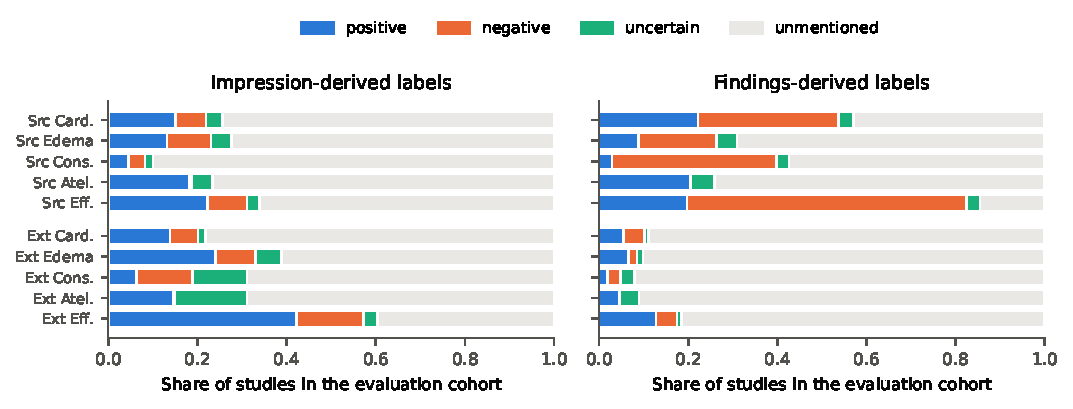
\includegraphics[width=\linewidth]{figures/fig2_label_composition.pdf}
\caption{Share of evaluation-cohort studies whose label for each target is
positive, negative, uncertain or unmentioned, by site and report section.
Values are in \cref{tab:labels}.}
\label{fig:labels}
\end{figure}

\subsection{The estimator defect and its correction}
\label{sec:res-defect}
Every original Stage 10 estimate was reproduced exactly from the cached
predictions. The original estimator counts each accepted study without a
labelled target as error-free, so its value is the error among evaluable
accepted studies multiplied by the evaluable fraction of accepted studies
(\cref{sec:endpoint}). That fraction is about 0.5 at the source and 0.8
externally, so the original estimator deflated source risk roughly twice as
much as external risk (\cref{tab:levels}). For M4 under intact context, the
original risks were \RiskOrigSrcMFour{} (source) and \RiskOrigExtMFour{}
(external); among evaluable studies they were \RiskEvalSrcMFour{} and
\RiskEvalExtMFour{}.

\begin{table}[t]
\centering\small
\caption{Selective error at the frozen 80\% cutoff under the original estimator
(label-less studies counted correct) and the corrected evaluable-study
estimator, with realised coverage over all eligible studies.}
\label{tab:levels}
\begin{adjustbox}{max width=\linewidth}
\begin{tabular}{llrrrrrr}
\toprule
 & & \multicolumn{3}{c}{Source} & \multicolumn{3}{c}{External}\\
\cmidrule(lr){3-5}\cmidrule(lr){6-8}
Model & Estimator & C0 & C1 & C2 & C0 & C1 & C2\\
\midrule
M1 & original (defective) & 0.1084 & 0.1084 & 0.1084 & 0.1818 & 0.1818 & 0.1818\\
 & evaluable-study & 0.2111 & 0.2111 & 0.2111 & 0.2230 & 0.2230 & 0.2230\\
 & \emph{coverage (all)} & 0.796 & 0.796 & 0.796 & 0.772 & 0.772 & 0.772\\
\addlinespace
M2 & original (defective) & 0.1575 & 0.2411 & 0.2415 & 0.2338 & 0.2605 & 0.2667\\
 & evaluable-study & 0.3042 & 0.4565 & 0.4618 & 0.2869 & 0.3203 & 0.3279\\
 & \emph{coverage (all)} & 0.803 & 1.000 & 0.790 & 0.847 & 1.000 & 0.846\\
\addlinespace
M3 & original (defective) & 0.1102 & 0.0951 & 0.1426 & 0.1571 & 0.1444 & 0.1676\\
 & evaluable-study & 0.1937 & 0.1755 & 0.2538 & 0.1895 & 0.1761 & 0.2024\\
 & \emph{coverage (all)} & 0.798 & 0.821 & 0.728 & 0.774 & 0.828 & 0.746\\
\addlinespace
M4 & original (defective) & 0.0744 & 0.0720 & 0.0893 & 0.1128 & 0.1200 & 0.1140\\
 & evaluable-study & 0.1391 & 0.1395 & 0.1695 & 0.1374 & 0.1466 & 0.1388\\
 & \emph{coverage (all)} & 0.800 & 0.805 & 0.789 & 0.795 & 0.764 & 0.788\\
\bottomrule
\end{tabular}

\end{adjustbox}
\end{table}

\subsection{Registered hypotheses}
\label{sec:res-hyp}
\Cref{tab:hyp} gives every Stage 10 contrast under both estimators with the
registered verdict rule. Under the corrected estimator, H1 was not confirmed
for either multimodal model: \HOneMThreeEval{} for M3 and \HOneMFourEval{} for
M4. Both intervals lie inside $(-0.02,0.02)$, so they exclude a material
increase at the realised calibration sample and model weights. Under the
original estimator the same contrasts were \HOneMThreeOrig{} and
\HOneMFourOrig{}, the original confirmation. H2 (C1) was not confirmed by
either estimator: \HTwoMThreeCOneEval{} for M3 and \HTwoMFourCOneEval{} for M4.
The registered H3 is identical to H2-C1 and is likewise not confirmed. The post
hoc transfer-gap version of H3 was negative for both models under both
estimators. Under the corrected estimator its magnitude is below materiality
(\HThreeMThreeEval{} and \HThreeMFourEval{}), so the ``reversal at
materiality'' of the previous draft does not survive correction.

Under its registered direction-only rule, H4 was supported for M3 at both sites
and for M4 at the source. For M4 externally, misaligned context gave lower
error than absent context (\HFourMFourexternalEval{}).

\begin{table}[t]
\centering\footnotesize
\begin{adjustbox}{max width=\linewidth}
\begin{tabular}{lllrlrl}
\toprule
H & Model & Contrast & \multicolumn{2}{c}{Original estimator} & \multicolumn{2}{c}{Corrected (evaluable-study)}\\
\cmidrule(lr){4-5}\cmidrule(lr){6-7}
 & & & Estimate (95\% CI) & V & Estimate (95\% CI) & V\\
\midrule
H1 & M3 & ext $-$ src, C0 & +0.0469 (+0.0408, +0.0531) & C & $-$0.0042 ($-$0.0145, +0.0061) & I\\
H1 & M4 & ext $-$ src, C0 & +0.0384 (+0.0336, +0.0430) & C & $-$0.0018 ($-$0.0108, +0.0064) & I\\
H2 & M3 & interaction, C1 & +0.0024 ($-$0.0027, +0.0076) & I & +0.0048 ($-$0.0038, +0.0134) & I\\
H2 & M4 & interaction, C1 & +0.0096 (+0.0048, +0.0144) & S & +0.0089 (+0.0002, +0.0173) & S\\
\midrule\multicolumn{7}{l}{\emph{H3 as coded after inspection (registered H3 $\equiv$ H2-C1)}}\\
H3 & M3 & gap $-$ gap(M1) & $-$0.0265 ($-$0.0321, $-$0.0212) & O [O*] & $-$0.0162 ($-$0.0256, $-$0.0070) & O [O]\\
H3 & M4 & gap $-$ gap(M1) & $-$0.0350 ($-$0.0408, $-$0.0292) & O [O*] & $-$0.0138 ($-$0.0243, $-$0.0029) & O [O]\\
\midrule\multicolumn{7}{l}{\emph{Secondary: H4 (direction only, no materiality)}}\\
H4 & M3 & C2 $-$ C1, source & +0.0475 (+0.0422, +0.0524) & C & +0.0783 (+0.0691, +0.0865) & C\\
H4 & M4 & C2 $-$ C1, source & +0.0173 (+0.0125, +0.0217) & C & +0.0301 (+0.0215, +0.0383) & C\\
H4 & M3 & C2 $-$ C1, external & +0.0231 (+0.0211, +0.0250) & C & +0.0263 (+0.0240, +0.0286) & C\\
H4 & M4 & C2 $-$ C1, external & $-$0.0060 ($-$0.0080, $-$0.0041) & O & $-$0.0077 ($-$0.0101, $-$0.0054) & O\\
\midrule\multicolumn{7}{l}{\emph{Not registered (computed by the original analysis code; descriptive)}}\\
H2 & M3 & interaction, C2 & $-$0.0219 ($-$0.0279, $-$0.0160) & O* & $-$0.0472 ($-$0.0572, $-$0.0374) & O*\\
H2 & M4 & interaction, C2 & $-$0.0137 ($-$0.0185, $-$0.0087) & O & $-$0.0289 ($-$0.0377, $-$0.0199) & O*\\
H1 & M1 & ext $-$ src, C0 & +0.0734 (+0.0668, +0.0802) & C & +0.0120 ($-$0.0002, +0.0244) & I\\
H1 & M2 & ext $-$ src, C0 & +0.0763 (+0.0687, +0.0838) & C & $-$0.0173 ($-$0.0292, $-$0.0054) & O\\
\bottomrule
\end{tabular}

\end{adjustbox}
\caption{All Stage 10 contrasts under the original and corrected estimators.
V: verdict under the registered rule (H1, H2: interval above zero and point
$\ge0.02$; H3: no materiality registered; H4: interval above zero). C
confirmed; S same direction, below materiality; I inconclusive (interval
includes zero); O opposite direction (below materiality, or no materiality
registered); O* opposite direction with magnitude $\ge0.02$. For H3 the bracket gives the verdict with the 0.02
materiality that the Stage 10 code applied. Rows marked not registered were
computed by the Stage 10 code but are not registered hypotheses.}
\label{tab:hyp}
\end{table}

\subsection{The cross-site contrast is not robust to defensible endpoint choices}
\label{sec:res-sensitivity}
\Cref{fig:spec} and \cref{tab:sens} show H1 under 15 specifications. Among
estimators that exclude label-less studies, the M4 transfer gap ranged from
\SensUncPosHOneMFour{} with uncertain labels counted as positive to
\SensUnmNegHOneMFour{} with unmentioned labels counted as negative. It was
\SensMacroHOneMFour{} under pathology-macro aggregation and
\SensFindHOneMFour{} with findings labels. Under the second training seed it was
\SensSeedHOneMFour{}, against \HOneMFourEval{} for the primary seed. The
original estimator gave \SensSeedOrigHOneMFour{} for that seed, which is why the
earlier replicate appeared to agree. For M3, retraining M2 under the second
seed (M3 averages M1 and M2) moved the corrected gap from \HOneMThreeEval{} to
\SensSeedHOneMThree{}. For M3, estimates ranged from
\SensTTenHOneMThreePt{} ($T=10$) to \SensUnmNegHOneMThreePt{} (unmentioned
counted as negative). No single factor dominated. Depending on the model, each
of the following moved the estimate by more than its own interval width:
aggregation (M1: \SensEvalHOneMOnePt{} evaluable-study against
\SensMacroHOneMOnePt{} pathology-macro), label handling (all models), label
source (M1 and M3) and training seed (M3 and M4).

The label-handling and aggregation specifications share the same predictions,
thresholds and cutoffs. Only which cells count as labelled, and how cells are
pooled, changes between them, and these choices alone decide the sign of the
cross-site contrast. Treating unmentioned cells
as negative brings the external site's lower specificity into view
(\cref{sec:res-operating}). The primary handling hides it, because labelled
external cells are mostly positive. Counting uncertain cells as positive does
the reverse for the same reason.

The pathology-specific contrasts that the original SAP made primary
(supplement) were heterogeneous. For M4 the primary labels gave cardiomegaly
\PathMFourCard{} and atelectasis \PathMFourAtel{}, while counting unmentioned as
negative made every pathology positive (\PathMFourUnmMin{} to
\PathMFourUnmMax{}). Restricted to AP-only studies, M4's
transfer gap was \ViewAPMFour{}; restricted to PA-only studies, \ViewPAMFour{}.
AP-only studies made up \APShareSrc{} of the source cohort and \APShareExt{} of
the external one, so view mix also enters the aggregate contrast.

\begin{figure}[t]
\centering
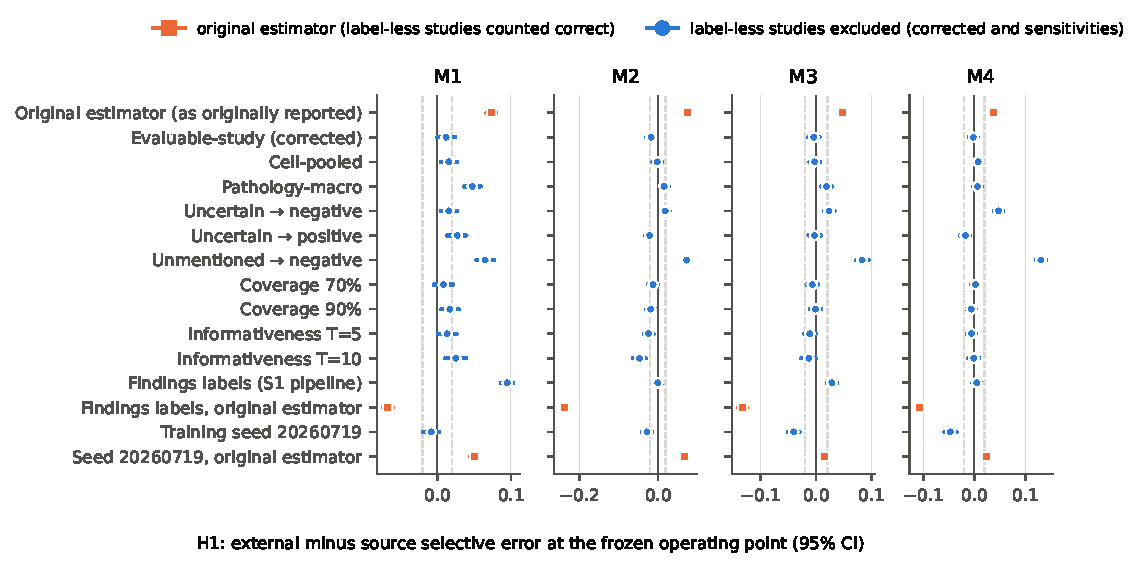
\includegraphics[width=\linewidth]{figures/fig1_h1_specifications.pdf}
\caption{H1 transfer gap (external minus source selective error, 95\% CI) for
each model under 15 specifications. Label-handling and aggregation rows share
the primary predictions, thresholds and cutoffs. Coverage rows change the
cutoff, $T$ rows the cohort, findings rows the labels, cohort and thresholds, and
seed rows the models. Square markers use the original estimator, which counts studies
without a labelled target as correct. Dashed lines mark $\pm0.02$. Values are
in \cref{tab:sens} and the supplement.}
\label{fig:spec}
\end{figure}

\begin{table}[t]
\centering\scriptsize
\caption{H1 and the post hoc transfer-gap H3 for the multimodal models across
specifications (point estimate and 95\% CI). Label-handling and aggregation rows
hold the primary predictions, thresholds and cutoffs fixed; the other rows change
the cutoff (coverage), the cohort ($T$), the labels, cohort and thresholds
(findings) or the models (seed).}
\label{tab:sens}
\begin{adjustbox}{max width=\linewidth}
\begin{tabular}{lrrrr}
\toprule
Specification & H1 M3 & H1 M4 & H3 M3 & H3 M4\\
\midrule
Original estimator (as originally reported) & +0.0469 (+0.041, +0.053) & +0.0384 (+0.034, +0.043) & $-$0.0265 ($-$0.032, $-$0.021) & $-$0.0350 ($-$0.041, $-$0.029)\\
Evaluable-study (corrected) & $-$0.0042 ($-$0.014, +0.006) & $-$0.0018 ($-$0.011, +0.006) & $-$0.0162 ($-$0.026, $-$0.007) & $-$0.0138 ($-$0.024, $-$0.003)\\
Cell-pooled & $-$0.0026 ($-$0.012, +0.007) & +0.0076 ($-$0.000, +0.015) & $-$0.0183 ($-$0.026, $-$0.010) & $-$0.0080 ($-$0.017, +0.001)\\
Pathology-macro & +0.0188 (+0.009, +0.029) & +0.0063 ($-$0.002, +0.014) & $-$0.0287 ($-$0.037, $-$0.020) & $-$0.0412 ($-$0.050, $-$0.032)\\
Uncertain $\to$ negative & +0.0232 (+0.014, +0.033) & +0.0475 (+0.039, +0.056) & +0.0075 ($-$0.001, +0.016) & +0.0319 (+0.022, +0.042)\\
Uncertain $\to$ positive & $-$0.0025 ($-$0.014, +0.008) & $-$0.0176 ($-$0.027, $-$0.009) & $-$0.0295 ($-$0.038, $-$0.020) & $-$0.0446 ($-$0.055, $-$0.034)\\
Unmentioned $\to$ negative & +0.0828 (+0.072, +0.094) & +0.1306 (+0.121, +0.141) & +0.0179 (+0.013, +0.023) & +0.0657 (+0.059, +0.073)\\
Coverage 70\% & $-$0.0069 ($-$0.017, +0.003) & +0.0029 ($-$0.006, +0.011) & $-$0.0150 ($-$0.025, $-$0.005) & $-$0.0052 ($-$0.016, +0.006)\\
Coverage 90\% & $-$0.0010 ($-$0.011, +0.009) & $-$0.0058 ($-$0.015, +0.002) & $-$0.0181 ($-$0.027, $-$0.009) & $-$0.0229 ($-$0.033, $-$0.012)\\
Informativeness $T=5$ & $-$0.0114 ($-$0.022, $-$0.001) & $-$0.0057 ($-$0.015, +0.003) & $-$0.0248 ($-$0.034, $-$0.015) & $-$0.0190 ($-$0.030, $-$0.008)\\
Informativeness $T=10$ & $-$0.0130 ($-$0.027, $-$0.000) & $-$0.0009 ($-$0.012, +0.010) & $-$0.0381 ($-$0.050, $-$0.026) & $-$0.0260 ($-$0.039, $-$0.012)\\
Findings labels (S1 pipeline) & +0.0285 (+0.019, +0.038) & +0.0048 ($-$0.003, +0.013) & $-$0.0666 ($-$0.074, $-$0.058) & $-$0.0903 ($-$0.098, $-$0.082)\\
Findings labels, original estimator & $-$0.1324 ($-$0.140, $-$0.125) & $-$0.1079 ($-$0.114, $-$0.101) & $-$0.0652 ($-$0.071, $-$0.058) & $-$0.0408 ($-$0.047, $-$0.034)\\
Training seed 20260719 & $-$0.0402 ($-$0.050, $-$0.030) & $-$0.0469 ($-$0.059, $-$0.035) & $-$0.0320 ($-$0.040, $-$0.024) & $-$0.0386 ($-$0.047, $-$0.030)\\
Seed 20260719, original estimator & +0.0145 (+0.009, +0.021) & +0.0246 (+0.018, +0.031) & $-$0.0366 ($-$0.041, $-$0.032) & $-$0.0265 ($-$0.032, $-$0.022)\\
\bottomrule
\end{tabular}

\end{adjustbox}
\end{table}

\subsection{Controlled label-source decomposition}
\label{sec:res-label-source}
The original findings-label sensitivity (S1) changed the label set, the
source cohort (14,766 to 9,293 studies), the thresholds and cutoffs (re-selected
on findings calibration labels), and the C2 donor realisation, all at once.
Model parameters did not change. External probabilities agreed between the two
runs to within \SOneMaxProbDiff{}. With S1's re-selected thresholds, however,
M1's external decisions differed in \SOneMOneCells{} cells and its acceptance in
\SOneMOneStudies{} studies, and across models \SOneCellsChanged{} cells and
\SOneStudiesChanged{} studies changed. The previous draft's argument that ``only
the labels differ'' for the image-only control was therefore incorrect.
\Cref{tab:ls} changes one factor at a time.

Swapping labels alone (A0$\to$A1) on the same studies, with identical
decisions and accepted sets, moved the original-estimator M3 contrast from
\LSAZeroMThreeOrig{} to \LSAOneMThreeOrig{}. Restricting the source cohort
(A1$\to$A2) moved it further, to \LSATwoMThreeOrig{}, because it removes
label-less source studies that the original estimator counted as correct.
Re-selecting thresholds (A2$\to$A3) reproduced the originally reported
\LSAThreeMThreeOrig{}. Under the corrected estimator the cohort restriction has
exactly no effect, because the removed studies are not evaluable under findings
labels. The remaining movement is shared between labels (A0$\to$A1:
\LSAZeroMThreeEval{} to \LSAOneMThreeEval{} for M3, and \LSAZeroMFourEval{} to
\LSAOneMFourEval{} for M4) and thresholds (A2$\to$A3: to \LSAThreeMThreeEval{} and
\LSAThreeMFourEval{}). On cells labelled under both sources (A1c), impression and
findings labels gave nearly the same contrasts: \LSAOnecIMThreeEval{} and
\LSAOnecFMThreeEval{} for M3. Under the corrected estimator, the findings-label
result does not reverse the primary; for M3 it points in the hypothesised
direction. The originally reported reversal under S1 was produced by the estimator defect
interacting with the asymmetric cohort definition, not by the label sets
measuring opposite things.

\begin{table}[t]
\centering\scriptsize
\caption{Controlled label-source decomposition of H1 (point estimates; intervals
in the supplement). Evaluable studies: share of each cohort with at least one
labelled target under that step's labels. Under the corrected estimator, A2
equals A1 because the studies removed by the cohort restriction are not
evaluable under findings labels.}
\label{tab:ls}
\begin{adjustbox}{max width=\linewidth}
\begin{tabular}{llrrrrrr}
\toprule
 & & \multicolumn{2}{c}{Evaluable studies} & \multicolumn{2}{c}{H1 M3} & \multicolumn{2}{c}{H1 M4}\\
\cmidrule(lr){3-4}\cmidrule(lr){5-6}\cmidrule(lr){7-8}
Step & Change from A0 & Src & Ext & Original & Corrected & Original & Corrected\\
\midrule
A0 & primary (impression labels, primary cohort, impression thresholds) & 53\% & 81\% & +0.0469 & $-$0.0042 & +0.0384 & $-$0.0018\\
A1 & findings labels only & 59\% & 24\% & $-$0.0613 & +0.0090 & $-$0.0839 & $-$0.0389\\
A1c-I & common labelled cells, impression labels & 20\% & 17\% & $-$0.0059 & $-$0.0042 & $-$0.0065 & $-$0.0212\\
A1c-F & common labelled cells, findings labels & 20\% & 17\% & $-$0.0069 & $-$0.0090 & $-$0.0077 & $-$0.0271\\
A2x & findings cohort only & 37\% & 81\% & +0.0809 & +0.0012 & +0.0664 & +0.0126\\
A2 & findings cohort + labels & 94\% & 24\% & $-$0.1359 & +0.0090 & $-$0.1610 & $-$0.0389\\
A3 & + findings thresholds and cutoffs (= original S1) & 94\% & 24\% & $-$0.1324 & +0.0285 & $-$0.1079 & +0.0048\\
B2 & findings labels + thresholds, primary cohort & 59\% & 24\% & $-$0.0579 & +0.0285 & $-$0.0524 & +0.0048\\
\bottomrule
\end{tabular}

\end{adjustbox}
\end{table}

\subsection{Frozen thresholds and per-pathology operating points}
\label{sec:res-operating}
Aggregate error hid a shift in operating points (\cref{tab:operating},
\cref{fig:operating}). For M4 among accepted studies, cardiomegaly specificity
fell from \MFourCardSpecSrc{} at the source to \MFourCardSpecExt{} externally
while sensitivity rose from \MFourCardSensSrc{} to \MFourCardSensExt{}. The
model called cardiomegaly in \MFourCardPosSrc{} of accepted studies at the
source and \MFourCardPosExt{} externally. Specificity also fell for effusion
(\MFourEffSpecSrc{} to \MFourEffSpecExt{}) and edema (\MFourEdemaSpecSrc{} to
\MFourEdemaSpecExt{}). Negative labels are explicit mentions and therefore a
selected subset, so these specificities carry verification bias. The direction
held when unmentioned cells were counted as negative (supplement). A frozen
threshold transferred a decision rule, not an operating point.

\begin{table}[t]
\centering\scriptsize
\caption{Per-pathology operating characteristics among accepted studies (C0),
labelled cells only. Pos.\ call: share of accepted studies in which the model
called the finding positive.}
\label{tab:operating}
\begin{adjustbox}{max width=\linewidth}
\begin{tabular}{lllrrrrrr}
\toprule
 & & & \multicolumn{3}{c}{Source} & \multicolumn{3}{c}{External}\\
\cmidrule(lr){4-6}\cmidrule(lr){7-9}
Model & Pathology & $t_j$ & Sens. & Spec. & Pos.\ call & Sens. & Spec. & Pos.\ call\\
\midrule
M3 & Cardiomegaly & 0.617 & 0.872 & 0.788 & 0.585 & 0.965 & 0.579 & 0.704\\
 & Edema & 0.575 & 0.840 & 0.806 & 0.389 & 0.808 & 0.749 & 0.539\\
 & Consolidation & 0.553 & 0.824 & 0.851 & 0.416 & 0.808 & 0.905 & 0.591\\
 & Atelectasis & 0.986 & 0.667 & 0.780 & 0.451 & 0.550 & 0.897 & 0.515\\
 & Pleural Effusion & 0.686 & 0.863 & 0.841 & 0.448 & 0.851 & 0.901 & 0.589\\
\addlinespace
M4 & Cardiomegaly & 0.633 & 0.887 & 0.823 & 0.563 & 0.972 & 0.438 & 0.756\\
 & Edema & 0.436 & 0.848 & 0.838 & 0.363 & 0.885 & 0.653 & 0.651\\
 & Consolidation & 0.584 & 0.841 & 0.889 & 0.376 & 0.805 & 0.915 & 0.531\\
 & Atelectasis & 0.964 & 0.886 & 0.460 & 0.724 & 0.911 & 0.498 & 0.875\\
 & Pleural Effusion & 0.798 & 0.870 & 0.887 & 0.487 & 0.950 & 0.641 & 0.751\\
\bottomrule
\end{tabular}

\end{adjustbox}
\end{table}

\begin{figure}[t]
\centering
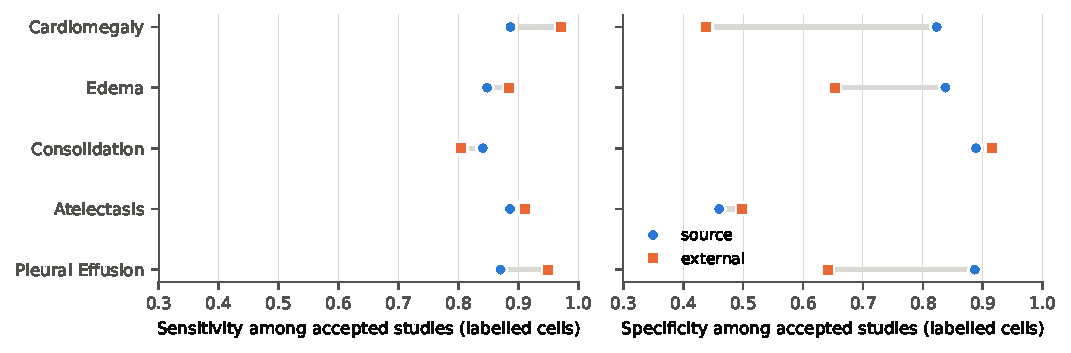
\includegraphics[width=\linewidth]{figures/fig4_operating_points.pdf}
\caption{M4 sensitivity and specificity among accepted studies at the source
(circles) and external site (squares), labelled cells only. Values in
\cref{tab:operating}.}
\label{fig:operating}
\end{figure}

\subsection{Coverage, the confidence score and alternative policies}
\label{sec:res-selective}
With context intact, realised coverage stayed within \CovDriftMaxCZero{} of the
80\% target for every model at both sites, and within \SeedCovDriftMax{} under
the second seed. Under intervention it moved: M2 under C1 accepted every study
at both sites (\MTwoCOneCovSrc{} and \MTwoCOneCovExt{}), because a constant
placeholder makes its output constant and every study ties at the same
confidence. M3 under C2 fell to \MThreeCTwoCovSrc{} and \MThreeCTwoCovExt{}.
Coverage held while per-pathology operating points shifted
(\cref{sec:res-operating}), so coverage monitoring alone would not reveal that
shift. Whether selective \emph{error} degraded is the question the labels could
not settle (\cref{sec:res-sensitivity}).

The frozen confidence score ranked study-level correctness only weakly:
failure-detection AUROC was \FailAUROCFrozenMin{}--\FailAUROCFrozenMax{} across
models and sites (\cref{fig:rc}, \cref{tab:comparators}). Three comparators
were fitted on the source calibration tier only. A per-pathology
temperature-scaled margin left the policy nearly unchanged. A decision-aware
expected-loss score, built from Platt-calibrated probabilities of error for the
decisions actually made, ranked errors better (AUROC
\FailAUROCELMin{}--\FailAUROCELMax{}) and lowered risk at both sites. Its
operating point transported worse: M4's external coverage was \ELMFourExtCov{}
against an 80\% calibration target. Split-conformal singleton acceptance with
one miscoverage level could not reach 80\% calibration coverage
(\ConfAccMin{}--\ConfAccMax{}), because near-uniformly positive atelectasis
labels make that pathology's sets rarely singleton. Its acceptance rate also
moved at the external site.

\begin{figure}[t]
\centering
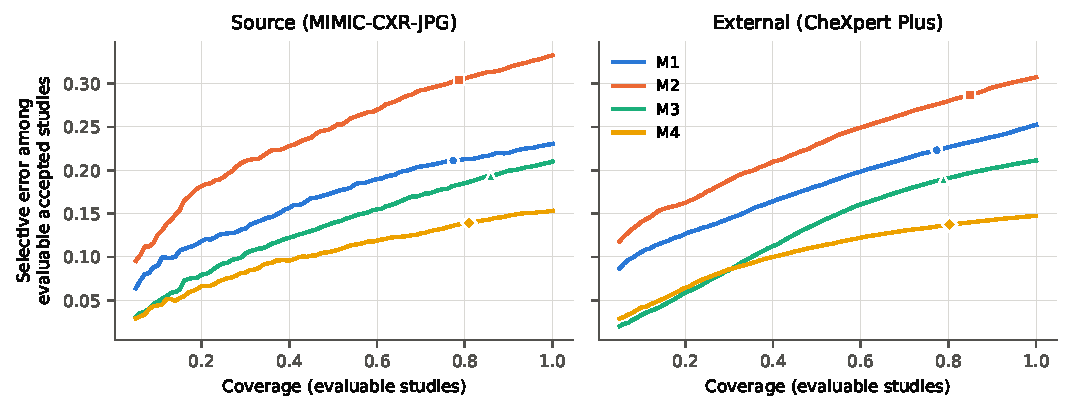
\includegraphics[width=\linewidth]{figures/fig3_risk_coverage.pdf}
\caption{Risk--coverage curves over evaluable studies (C0), ranking by the
frozen confidence score. Markers show the frozen 80\% operating point at its
realised coverage among evaluable studies.}
\label{fig:rc}
\end{figure}

\begin{table}[t]
\centering\scriptsize
\caption{Alternative selective policies (post hoc), all fitted on the source
calibration tier and applied unchanged. Failure AUROC: discrimination of
studies with no error versus any error, evaluable studies. H1 corrected:
evaluable-study transfer gap.}
\label{tab:comparators}
\begin{adjustbox}{max width=\linewidth}
\begin{tabular}{llrrrrrr}
\toprule
 & & \multicolumn{2}{c}{Coverage (C0)} & \multicolumn{2}{c}{Failure AUROC} & & \\
\cmidrule(lr){3-4}\cmidrule(lr){5-6}
Model & Policy & Src & Ext & Src & Ext & H1 corrected (95\% CI) & Ext.\ coverage C1\\
\midrule
M3 & Frozen (|2p$-$1|) & 0.798 & 0.774 & 0.632 & 0.648 & $-$0.0042 ($-$0.014, +0.006) & 0.828\\
 & Temperature-scaled margin & 0.798 & 0.772 & 0.633 & 0.652 & $-$0.0042 ($-$0.015, +0.006) & 0.827\\
 & Expected-loss (decision-aware) & 0.797 & 0.733 & 0.738 & 0.746 & $-$0.0166 ($-$0.026, $-$0.007) & 0.777\\
 & Split-conformal singletons & 0.515 & 0.552 & 0.643 & 0.697 & $-$0.0205 ($-$0.029, $-$0.013) & 0.572\\
\addlinespace
M4 & Frozen (|2p$-$1|) & 0.800 & 0.795 & 0.625 & 0.603 & $-$0.0018 ($-$0.011, +0.006) & 0.764\\
 & Temperature-scaled margin & 0.800 & 0.796 & 0.627 & 0.604 & $-$0.0018 ($-$0.011, +0.006) & 0.762\\
 & Expected-loss (decision-aware) & 0.800 & 0.855 & 0.704 & 0.687 & +0.0056 ($-$0.002, +0.013) & 0.937\\
 & Split-conformal singletons & 0.559 & 0.693 & 0.644 & 0.664 & +0.0290 (+0.021, +0.037) & 0.701\\
\bottomrule
\end{tabular}

\end{adjustbox}
\end{table}

\subsection{Context interventions within each site}
\label{sec:res-context}
For M3, misaligned context (C2) gave higher error than absent context (C1) at
the source under every estimator, label variant, coverage, informativeness
threshold, label source, C2 permutation and both training seeds
(\HFourMThreesourceEval{} for the primary seed, \RepTwoHFourMThreesourceeval{}
for the second). At the external site it did so under every specification for
the primary seed (\HFourMThreeexternalEval{}), and an alternative C2 donor
permutation left it essentially unchanged (range \PermHFourMThreeExtRange{}
across the two permutations). Under the second training seed the
corrected estimate was \RepTwoHFourMThreeexternaleval{}, inconclusive, and the
original estimator gave \RepTwoHFourMThreeexternalorig{}. For M4 the effect was positive at the
source (\HFourMFoursourceEval{}) in all primary-seed specifications, but the
interval included zero under the second seed. Externally its sign depended on
label handling. Removing or replacing context mostly changed predictions rather
than selection (\cref{tab:context}). Even so, the accepted sets under C0 and
under intervention overlapped only partially (Jaccard
\JaccardMin{}--\JaccardMax{}), so paired conditions do not evaluate the same
accepted studies. The two orderings of the selection/prediction split
disagreed by up to \OrderGapMM{} for the multimodal models (\OrderGapMTwo{} for M2), so no unique
additive split exists. The C2
interaction was negative for both multimodal models under the primary labels
(\HTwoMThreeCTwoEval{} and \HTwoMFourCTwoEval{}), meaning misalignment cost less
externally. This is consistent with the shorter external contexts (mean
\CTwoTokensExt{} versus \CTwoTokensSrc{} effective tokens), of which C2 changed
the target-term content in \CTwoTermDiffExt{} of external rows against
\CTwoTermDiffSrc{} at the source. The C2 interaction is not a registered
hypothesis, and its sign reversed when unmentioned cells were counted as
negative.

\begin{table}[t]
\centering\scriptsize
\caption{Selection versus prediction under context interventions (corrected
estimator). Policy effect $=R_c(A_c)-R_0(A_0)$; prediction on C0 set
$=R_c(A_0)-R_0(A_0)$; selection (o1) $=R_c(A_c)-R_c(A_0)$; selection (o2)
$=R_0(A_c)-R_0(A_0)$; Jaccard overlap of $A_0$ and $A_c$. Intervals in the
supplement.}
\label{tab:context}
\begin{adjustbox}{max width=\linewidth}
\begin{tabular}{lllrrrrr}
\toprule
Site & Model & Cond. & Policy effect & Pred.\ on C0 set & Selection (o1) & Selection (o2) & Jaccard\\
\midrule
source & M3 & C1 & $-$0.0182 & $-$0.0181 & $-$0.0001 & +0.0075 & 0.69\\
 & M3 & C2 & +0.0601 & +0.0714 & $-$0.0113 & +0.0148 & 0.64\\
 & M4 & C1 & +0.0003 & +0.0000 & +0.0003 & +0.0054 & 0.68\\
 & M4 & C2 & +0.0304 & +0.0333 & $-$0.0029 & +0.0079 & 0.68\\
\addlinespace
external & M3 & C1 & $-$0.0134 & $-$0.0127 & $-$0.0007 & +0.0063 & 0.68\\
 & M3 & C2 & +0.0129 & +0.0157 & $-$0.0029 & +0.0077 & 0.67\\
 & M4 & C1 & +0.0092 & +0.0132 & $-$0.0040 & +0.0011 & 0.65\\
 & M4 & C2 & +0.0015 & +0.0031 & $-$0.0017 & +0.0002 & 0.68\\
\bottomrule
\end{tabular}

\end{adjustbox}
\end{table}

\subsection{Sources of uncertainty the evaluation bootstrap omits}
\label{sec:res-uncertainty}
Resampling calibration patients and re-applying the frozen selection rule moved
the corrected H1 estimates with a standard deviation \CalRatioMin{}--\CalRatioMax{}
times the evaluation-bootstrap standard deviation (\cref{tab:uncertainty}). For
M4 the calibration standard deviation was \CalSDMFour{} against \EvalSDMFour{}, and
per-pathology thresholds varied with standard deviation up to \ThrSDMaxMFour{}.
The training seed moved the corrected H1 of both multimodal models by about
0.04 (\cref{sec:res-sensitivity}). The reported intervals, which condition on
one calibration sample and one training run, therefore understate total
uncertainty substantially for cross-site contrasts.

\begin{table}[t]
\centering\scriptsize
\caption{H1 variability from resampling evaluation patients (bootstrap SD,
approximated from the 95\% interval) and from resampling calibration patients
with the frozen selection rule re-applied (200 replicates).}
\label{tab:uncertainty}
\begin{adjustbox}{max width=\linewidth}
\begin{tabular}{llrrrr}
\toprule
Model & Estimator & H1 & SD (evaluation bootstrap) & SD (calibration resample) & Calibration 2.5--97.5\%\\
\midrule
M1 & original & +0.0734 & 0.0034 & 0.0044 & (+0.0635, +0.0845)\\
 & evaluable-study & +0.0120 & 0.0063 & 0.0092 & ($-$0.0003, +0.0388)\\
M2 & original & +0.0763 & 0.0038 & 0.0067 & (+0.0740, +0.0984)\\
 & evaluable-study & $-$0.0173 & 0.0061 & 0.0205 & ($-$0.0254, +0.0408)\\
M3 & original & +0.0469 & 0.0031 & 0.0050 & (+0.0352, +0.0554)\\
 & evaluable-study & $-$0.0042 & 0.0053 & 0.0097 & ($-$0.0271, +0.0141)\\
M4 & original & +0.0384 & 0.0024 & 0.0032 & (+0.0316, +0.0440)\\
 & evaluable-study & $-$0.0018 & 0.0044 & 0.0102 & ($-$0.0286, +0.0102)\\
\bottomrule
\end{tabular}

\end{adjustbox}
\end{table}

\subsection{Integrity checks and exploratory strata}
\label{sec:res-c2}
The previous draft reported 6 source and 34 external studies ``retaining their
own context'' under C2. Replaying the assignment, verified to reproduce it
exactly, showed that every one of these rows received identical text donated by
a \emph{different} patient. No recipient received context from its own patient
(\CTwoSamePatSrc{} and \CTwoSamePatExt{} same-patient donors). The count was a
count of identical boilerplate, not of constraint violations. Image-only
predictions were identical across conditions at both sites.

Among external demographic groups (exploratory; no source demographics were
available), M4's coverage differed by at most \AgeCovDispMFour{} across age bands
and \InsCovDispMFour{} across insurance categories. M3's coverage differed by \AgeCovDispMThree{}
across age bands, which exceeds the 0.05 drift materiality (supplement). These
are single-site, post hoc descriptions with no cross-site comparison.
